%%%%%%%%%%%%%%%%%%%%%%%%%%%%%%%%%%%%%%%%%%%%%%%%%%%%%%%%%%%%%%%%%%%%%%%%%%%%%%%%%%%%%%%%%%%%%%%%%%%
\documentclass[11pt]{beamer}
\usetheme{metropolis}
\usepackage[utf8]{inputenc}
\usepackage[spanish]{babel}
\usepackage{amsmath}
\usepackage{amsfonts}
\usepackage{amssymb}
\usepackage{graphicx}

% numeros con punto decimal, no coma
\decimalpoint

% para la bibliografia
\usepackage[style=verbose,backend=bibtex]{biblatex}
\bibstyle{abbrv}

% codigo de R
\usepackage{listings}
\usepackage{color}

% para las tablitas
\usepackage{booktabs}

% para tablas de colores
\usepackage{xcolor,colortbl}
\usepackage{multirow}

%\usefonttheme[onlymath]{mathserif}
%\usepackage{mathpazo} 
\usepackage{eulervm}                 %
\usepackage[scaled ]{helvet}  

\newcommand{\bordes}[1]{\renewcommand{\arraystretch}{#1}}
\definecolor{gray}{rgb}{0.5,0.5,0.5}
\definecolor{gris}{gray}{0.925}
\definecolor{gris2}{gray}{0.8}

%%%%%%%%%%%%%%%%%%%%%%%%%%%%%%%%%%%%%%%%%%%%%%%%%%%%%%%%%%%%%%%%%%%%%%%%%%%%%%%%%%%%%%%%%%%%%%%%%%%

\addbibresource{referencias_estacionariedad.bib}
\addbibresource{referencias_fisiologia.bib}
\addbibresource{referencias_otros.bib}
\addbibresource{referencias_mixto.bib}

\renewcommand{\footnotesize}{\tiny}

\newtheorem{defn}{Definici\'on}
\newtheorem{thrm}{Teorema}
\newtheorem{demostracion}{Demostraci\'on}
\newtheorem{prop}{Proposici\'on}

\newcommand{\R}{\mathbb{R}}
\newcommand{\intR}{\int_{-\infty}^{\infty}}
\newcommand{\intZ}{\int_{-\infty}^{0}}
\newcommand{\intPI}{\int_{-\pi}^{\pi}}
\newcommand{\simint}[1]{\int_{- #1 }^{ #1 }}
\newcommand{\prima}{^{\prime}}

\newcommand{\ddd}{$\delta$}
\newcommand{\dirac}{$\delta$  de Dirac}

\newcommand{\aste}[1]{\widehat{ #1 }^{\star}}
\newcommand{\est}[1]{\widehat{ #1 }}

\newcommand{\COS}[1]{\mathrm{cos}\left( #1 \right)}
\newcommand{\SEN}[1]{\mathrm{sen}\left( #1 \right)}

\newcommand{\E}[1]{\mathrm{E}\left[ #1 \right]}
\newcommand{\Var}[1]{\mathrm{Var}\left( #1 \right)}
\newcommand{\Cov}[1]{\mathrm{Cov}\left( #1 \right)}
\newcommand{\abso}[1]{\left| #1 \right|}

%%%%%%%%%%%%%%%%%%%%%%%%%%%%%%%%%%%%%%%%%%%%%%%%%%%%%%%%%%%%%%%%%%%%%%%%%%%%%%%%%%%%%%%%%%%%%%%%%%%

\author{Julio Cesar Enciso Alva}
\title{Estacionariedad d\'ebil}
\subtitle{Detecci\'on en series electrofisiol\'ogicas}
%\setbeamercovered{transparent} 
\setbeamertemplate{navigation symbols}{} 
%\logo{} 
\institute{Instituto de Ciencias B\'asicas e Ingenier\'ia\\ 
Universidad Aut\'onoma del Estado de Hidalgo} 
\date{\emph{Neuroscience Short Course}\\
6 de julio de 2017} 
%\subject{} 

%%%%%%%%%%%%%%%%%%%%%%%%%%%%%%%%%%%%%%%%%%%%%%%%%%%%%%%%%%%%%%%%%%%%%%%%%%%%%%%%%%%%%%%%%%%%%%%%%%%

\begin{document}

\begin{frame}
\titlepage
\end{frame}

%\begin{frame}
%\tableofcontents
%\end{frame}

\section{Introducci\'on}

%\subsection{Antecedentes}

%%%%%%%%%%%%%%%%%%%%%%%%%%%%%%%%%%%%%%%%%%%%%%%%%

%\begin{frame}\frametitle{Antecedentes}
%\begin{itemize}
%\item Encuesta Intercensal 2015 (INEGI): 12,500,000 adultos mayores, 10.4 \%  de la poblaci\'on 
%\footcite{Intercensal15}
%
%\item Posible relaci\'on trastornos del sue\~no y DC en la vejez \footcite{Miyata13}
%
%\item Epidemiolog\'ia del DC en Hidalgo: eficiencia del sue\~no \footcite{VazquezTagle16}
%
%\item DFA en registros de PSG \footcite{Valeria}: exponente de Hurst diferente en sujetos con y 
%sin DC 
%
%\item Se buscan marcadores cl\'inicos para el diagn\'ostico de DC
%\end{itemize}
%\end{frame}

\begin{frame}\frametitle{Motivaci\'on}
El estudio y diagnóstico de una gran cantidad de enfermedades depende de nuestra habilidad para
registrar y analizar se\~nales electrofisiol\'ogicas. \\

%\vspace{3em}
\vspace{2em}

Se suele asumir que estas se\~nales son complejas: no lineales, no estacionarias y sin equilibrio 
por naturaleza. Pero usualmente no se comprueban formalmente estas propiedades.
\end{frame}

\subsection{Matem\'aticas}

\begin{frame}\frametitle{Conceptos}
\begin{defn}[Estacionariedad d\'ebil]
Un proceso estoc\'astico es d\'ebilmente estacionario si y s\'olo si para cualesquiera tiempos 
admisibles $t$, $s$ se tiene que
\begin{itemize}
\item $\E{X(t)} = \mu_X$
\item $\Var{X(t)} = \sigma^{2}_X$
\item $\Cov{X(t),X(s)} = \rho_X (s-t)$
\end{itemize}
Con $\mu_X$, $\sigma^{2}_X$ constantes, $\rho_X(\tau)$ \'unicamente depende de $\tau$
\end{defn}
\end{frame}

\begin{frame}\frametitle{Conceptos}
\begin{defn}[Funci\'on de densidad espectral (SDF)]
Sea $\{X(t)\}$ un proceso estoc\'astico a tiempo continuo, d\'ebilmente estacionario
\begin{equation*}
h(\omega) = \lim_{T\rightarrow \infty} \E{ \frac{ \left| G_T(\omega) \right|^{2}}{2 T} }
\end{equation*}
Donde $\displaystyle G_T (\omega) = \frac{1}{\sqrt{2 \pi}} \int_{-T}^{T} X(t) e^{-i \omega t} dt$
\end{defn}
\end{frame}

\begin{frame}%\frametitle{}
\begin{thrm}[Wiener-Khinchin]
Una condici\'on suficiente y necesaria para que $\rho$ sea funci\'on de autocorrelaci\'on para 
alg\'un proceso a tiempo continuo d\'ebilmente estacionario y estoc\'asticamente continuo, 
$\{X(t)\}$,  es que exista una funci\'on $F$ tal que
\begin{itemize}
\item Es mon\'otonamente creciente
\item $F(-\infty) = 0$
\item $F(+\infty) = 1$
\item Para todo $\tau \in \R$ se cumple que
\begin{equation*}
\rho(\tau) = \intR e^{i \omega \tau} dF(\omega)
\end{equation*}
\end{itemize}
\end{thrm}
\end{frame}

\begin{frame}\frametitle{Espectro evolutivo}
Se consideran procesos no-estacionarios, estoc\'asticamente continuos, de media cero y varianza 
finita, y que admitan una representaci\'on de la forma
\begin{equation*}
X(t) = \intPI A(t,\omega) e^{i t \omega} dZ(\omega)
\end{equation*}
tal que 
\begin{itemize}
\item $\Cov{dZ(\omega),dZ(\lambda)} = 0 \Leftrightarrow \omega \neq \lambda$
\item $\E{\abso{dZ(\omega)}^{2}} = \mu(\omega)$
\end{itemize}

El \textbf{espectro evolutivo} fue definido por Priestley \footcite{Priestley65} como
\begin{equation*}
f(t,\omega) = \abso{A(t,\omega)}^{2}
\end{equation*}
\end{frame}

\begin{frame}%\frametitle{Estimador de doble ventana}
\begin{defn}[Estimador de doble ventana]
Se define a $\est{f}$, estimador para la $f$, como
\begin{equation*}
\widehat{f}(t,\omega) = \int_{t-T}^{t} w_{T'}(u) \lvert U(t-u,\omega) \lvert^{2} du
\end{equation*}

\begin{itemize}
\item $U(t,\omega) = \int_{t-T}^{t} g(u) X({t-u}) e^{i \omega (t-u)} du$

\item $2\pi \int_{-\infty}^{\infty} \lvert g(u) \lvert^{2} du = 
\int_{-\infty}^{\infty} \lvert \Gamma(\omega) \lvert^{2} d\omega = 1$
\item $w_{\tau}(t) \geq 0$ para cualesquiera $t$, $\tau$
\item $w_{\tau}(t) \rightarrow 0$ cuando $\lvert t \lvert \rightarrow \infty$, para todo $\tau$
\item $\int_{-\infty}^{\infty} w_{\tau}(t) dt = 1$ para todo $\tau$
\item $ \int_{-\infty}^{\infty} \left( w_{\tau}(t) \right)^{2} dt < \infty$ para todo $\tau$
\item $\exists C$ tal que  
$ \lim_{\tau\rightarrow\infty} \tau \int_{-\infty}^{t} \abso{ W_{\tau}(\lambda) }^{2} d\lambda = C$
\end{itemize}
\end{defn}
\end{frame}

%\begin{lrbox}{\mybox}%
%\begin{lstlisting}[caption={}]
%Priestley-Subba Rao stationarity Test for datos
%-----------------------------------------------
%Samples used              : 3072 
%Samples available         : 3069 
%Sampling interval         : 1 
%SDF estimator             : Multitaper 
%  Number of (sine) tapers : 5 
%  Centered                : TRUE 
%  Recentered              : FALSE 
%Number of blocks          : 11 
%Block size                : 279 
%Number of blocks          : 11 
%p-value for T             : 0.4130131 
%p-value for I+R           : 0.1787949 
%p-value for T+I+R         : 0.1801353 
%\end{lstlisting}
%\end{lrbox}%
%
%\begin{frame}[fragile]
%\begin{figure}
%\scalebox{0.8}{\usebox{\mybox}}
%\caption{La prueba de Priestley-Subba Rao se encuentra implementada en R como la funci\'on 
%\texttt{stationarity()}, del paquete \texttt{fractal}}
%\end{figure}
%\end{frame}

%%%%%%%%%%%%%%%%%%%%%%%%%%%%%%%%%%%%%%%%%%%%%%%%%

%\begin{frame}{Algo}
%Texto de ejemplo
%\end{frame}

%\begin{frame}{•}
%
%\end{frame}

\section{Metodolog\'ia}

%%%%%%%%%%%%%%%%%%%%%%%%%%%%%%%%%%%%%%%%%%%%%%%%%%%%%%%%%%%%%%%%%%%%%%%%%%%%%%%%%%%%%%%%%%%%%%%%%%%

\subsection{Sujetos}

%%%%%%%%%%%%%%%%%%%%%%%%%%%%%%%%%%%%%%%%%%%%%%%%%
%%%%%%%%%%%%%%%%%%%%%%%%%%%%%%%%%%%%%%%%%%%%%%%%%

\begin{frame}\frametitle{Sujetos}
Criterios de inclusi\'on:
\begin{itemize}
\item Firma del consentimiento informado
\item Edad entre 60 y 85 a\~nos
\item Diestros (mano derecha dominante)
\item Sin ansiedad, depresi\'on o s\'indromes focales
\item No usar medicamentos o sustancias para dormir
\item Voluntario para el registro de PSG
\end{itemize}

\textbf{9 participantes: 4 control, 5 PDC}
\end{frame}

%%%%%%%%%%%%%%%%%%%%%%%%%%%%%%%%%%%%%%%%%%%%%%%%%
%%%%%%%%%%%%%%%%%%%%%%%%%%%%%%%%%%%%%%%%%%%%%%%%%

\begin{frame}\frametitle{Sujetos}
\begin{table}
\centering
\bordes{1.1}
\begin{tiny}
\begin{tabular}{llcrrrrrrr}
\toprule
 \phantom{mm}&
 & \textbf{Sexo} & \textbf{Edad} & \textbf{Esc.} & \textbf{Neuropsi} & \textbf{MMSE} & \textbf{SATS} & \textbf{KATZ} & \textbf{Gds} \\
\midrule
\multicolumn{6}{l}{\textbf{Gpo. Control}}\\
&VCR    & F    & 59   & 12   & 107      & 29   & 21   & 0    & 3 \\
&MJH    & F    & 72   & 9    & 113      & 30   & 18   & 0    & 0 \\
&JAE    & F    & 78   & 5    & 102      & 28   & 19   & 0    & 5 \\
&GHA    & M    & 65   & 9    & 107.5    & 30   & 23   & 0    & 7 \\
&MFGR   & F    & 67   & 11   & 110      & 30   & 18   & 0    &   \\
\rowcolor{gris}
&\multicolumn{1}{c}{$\widehat{\mu}$} & 
              & 68.20& 9.20 & 107.90   & 29.40& 19.80& 0.00 & 3.00\\
\rowcolor{gris}
&\multicolumn{1}{c}{$\widehat{\sigma}$} & 
              & 7.19 & 2.68 & 4.07     & 0.89 & 2.17 & 0.00 & 3.08\\
\midrule
%\hline
\multicolumn{6}{l}{\textbf{Gpo. PDC}}\\
&CLO    & F    & 68   & 5    & 81       & 28   & 22   & 1    & 6 \\
&RLO    & F    & 63   & 9    & 90       & 29   & 20   & 0    & 3 \\
&RRU    & M    & 69   & 9    & 85       & 27   & 10   & 0    & 3 \\
&JGZ    & M    & 65   & 11   & 87       & 25   & 20   & 0    & 1 \\
\rowcolor{gris}
&\multicolumn{1}{c}{$\widehat{\mu}$} & 
              & 66.25& 8.50 & 85.75   & 27.25& 18.00& 0.25 & 3.25\\
\rowcolor{gris}
&\multicolumn{1}{c}{$\widehat{\sigma}$} & 
              & 2.75 & 2.52 & 3.77    & 1.71 & 5.42 & 0.50 & 2.06\\
\midrule
%\hline
\multicolumn{6}{l}{\textbf{Sujetos excluidos}}\\
&FGH    & M    & 71   & 9    & 83.5     & 21   & 23   & 0    & 4  \\
&MGG    & F    & 61   & 9    & 114      & 28   & 29   & 1    & 14 \\
&EMT    & M    & 50   & 22   & 106      & 30   & 15   & 0    & 4  \\
\bottomrule
\end{tabular} 
\end{tiny}
\end{table}
\end{frame}

\begin{frame}\frametitle{Gracias por su atenci\'on}
\begin{figure}
\centering
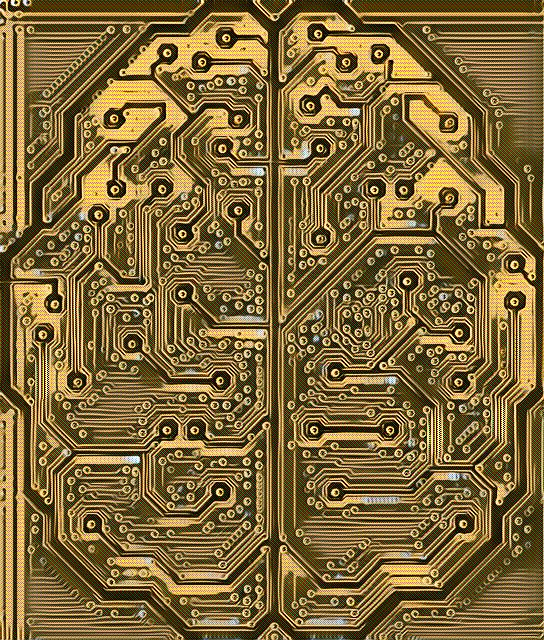
\includegraphics[width=0.4\linewidth]{./img_adornos/cerebot.jpg}\\
\vspace*{1em}
\textit{El cerebro es, quiz\'a, el \'unico \'organo capaz de estudiarse a s\'i mismo.}
\end{figure}
\end{frame}

%%%%%%%%%%%%%%%%%%%%%%%%%%%%%%%%%%%%%%%%%%%%%%%%%%%%%%%%%%%%%%%%%%%%%

\end{document}

%%%%%%%%%%%%%%%%%%%%%%%%%%%%%%%%%%%%%%%%%%%%%%%%%%%%%%%%%%%%%%%%%%%%%%%%%%%%%%%%%%%%%%%%%%%%%%%%%%%